\documentclass{beamer}

\input{settings.tex}


\title{Duality, Sensitivity, KKT}
\subtitle{\mycoursetitle, Lecture 13}
\author{by Sergei Savin}
\centering
\date{\mydate}



\begin{document}
\maketitle


%\begin{frame}{Content}
%
%\begin{itemize}
%\item Lagrange dual function
%\item Duality gap, strong and weak duality
%\item KKT conditions
%\item Sensitivity
%\end{itemize}
%
%\end{frame}







\begin{frame}{Lagrangian}
	\begin{flushleft}
		
		Consider an optimization problem:
		
		\begin{equation}
			\begin{aligned}
				& \underset{\bo{x}}{\text{minimize}}
				& & f_0(\bo{x}), \\
				& \text{subject to}
				& & \begin{cases}
					f_i(\bo{x}) \leq 0, \\
					h_j(\bo{x}) = 0.
				\end{cases}
			\end{aligned}
		\end{equation}
		
		It's \emph{Lagrangian} is given as:
		
		\begin{equation}
			L(\bo{x}, \lambda_i, \nu_j) = 
			f_0(\bo{x}) + 
			\sum\limits_i \lambda_i f_i(\bo{x}) +
			\sum\limits_j \nu_j h_j(\bo{x})
		\end{equation}
	%
	where $\lambda_i \geq 0$ and $\nu_j$ are Lagrange multipliers; they are sometimes called \emph{dual variables}.
		
	\end{flushleft}
\end{frame}




\begin{frame}{KKT conditions}
	\begin{flushleft}
		
		Karush-Kuhn-Tucker (KKT) conditions certify optimality of an optimization problem:
		
		\begin{equation}
			\begin{aligned}
				& \underset{\bo{x}}{\text{minimize}}
				& & f_0(\bo{x}), \\
				& \text{subject to}
				& & \begin{cases}
					f_i(\bo{x}) \leq 0, \\
					h_j(\bo{x}) = 0.
				\end{cases}
			\end{aligned}
		\end{equation}
		
		\begin{enumerate}
			\item Primal feasibility: $f_i(\bo{x}) \leq 0$ and $h_j(\bo{x}) = 0$.
			
			\item Dual feasibility: $\lambda_i \geq 0$.
			
			\item Complementarity slackness: $\lambda_i f_i(\bo{x}) = 0$.
			
			\item Lagrangian stationarity: $\frac{\partial}{\partial \bo{x}} 
			\left ( f_0(\bo{x}) + 
			\sum\limits_i \lambda_i f_i(\bo{x}) +
			\sum\limits_j \nu_j h_j(\bo{x}) \right ) = 0$.
		\end{enumerate}
		
	\end{flushleft}
\end{frame}




\begin{frame}{Lagrange dual function}
	\begin{flushleft}
		
	Given \emph{Lagrangian} $L(\bo{x}, \lambda_i, \nu_j) = 
	f_0(\bo{x}) + 
	\sum\limits_i \lambda_i f_i(\bo{x}) +
	\sum\limits_j \nu_j h_j(\bo{x})$, the associated 
	 \emph{Lagrange dual function} is given as:
		
		\begin{equation}
			g(\lambda_i, \nu_j)  = \underset{\bo{x}}{\text{inf}}
			\ L(\bo{x}, \lambda_i, \nu_j).
		\end{equation}
		
		Lagrange dual function is \textbf{always concave}. If $p^*$ is the optimal value of the cost function of the original problem, then $g(\lambda_i, \nu_j)$ gives as a \emph{lower bound} on its possible values:
		
		\begin{equation}
			g(\lambda_i, \nu_j)  \leq L(\bo{x}^*, \lambda_i, \nu_j)  \leq f_0(\bo{x}^*)
		\end{equation}
		
		In fact, substituting any $\nu_j$ and $\lambda_i \geq 0$ gives us a valid lower bound on the cost. Maximum of $g(\lambda_i, \nu_j)$ over the domain given by $\lambda_i \geq 0$ provides us the optimal (largest) lower bound of the problem, denoted as $g^*$. 
		
	\end{flushleft}
\end{frame}



\begin{frame}{Duality gap, strong and weak duality}
	\begin{flushleft}
		
		If $p^*$ is the optimal value of the cost function of the original problem and $g^*$ is the optimal lower bound of the problem, then $p^* - g^*$ is called optimal \emph{duality gap}.
		
		\bigskip
		
		If optimal duality gap is zero, the problem is said to have \emph{strong duality}. If optimal duality gap greater than zero, the problem is said to have \emph{weak duality}.
		
	\end{flushleft}
\end{frame}



\begin{frame}{Lagrange dual function for a QP, 1}
	\begin{flushleft}
		
		Consider the following QP:
		
		\begin{equation}
			\begin{aligned}
				& \underset{\bo{x}}{\text{minimize}}
				& & \bo{x}^\top \bo{H} \bo{x}, \\
				& \text{subject to}
				& & \bo{A}\bo{x} \leq \bo{b}.
			\end{aligned}
		\end{equation}
		%
		Its Lagrangian is:
		%
		\begin{equation}
			L(\bo{x}, \lambda) = \bo{x}^\top \bo{H} \bo{x} + \lambda^\top (\bo{A}\bo{x} - \bo{b})
		\end{equation}
		
		In order to minimize the Lagrangian with respect to $\bo{x}$ we find the gradient and set it to zero:
		%
		\begin{equation}
			\frac{\partial L(\bo{x}, \lambda)}{\partial \bo{x}} = 2\bo{x}^\top \bo{H} + \lambda^\top \bo{A} = 0
		\end{equation}
		
		With that we can compute $\bo{x}$ as a function of $\lambda$:
		%
		\begin{equation}
			\bo{x} = -0.5\bo{H}^{-1}\bo{A}^\top \lambda
		\end{equation}
		
	\end{flushleft}
\end{frame}



\begin{frame}{Lagrange dual function for a QP, 2}
	\begin{flushleft}
		
		Knowing that $\bo{x} = -0.5\bo{H}^{-1}\bo{A}^\top \lambda$ we can compute $g(\lambda)$ by substituting the $\bo{x}$ we found into the Lagrangian:
		%
		\begin{equation}
			g(\lambda) = \frac{1}{4} \lambda^\top \bo{A}\bo{H}^{-1}\bo{H}\bo{H}^{-1}\bo{A}^\top\lambda - \frac{1}{2} \lambda^\top \bo{A}\bo{H}^{-1}\bo{A}^\top \lambda - \lambda^\top\bo{b}
		\end{equation}
	%
	\begin{equation}
		g(\lambda) = -\frac{1}{4} \lambda^\top \bo{A}\bo{H}^{-1}\bo{A}^\top\lambda - \lambda^\top\bo{b}
	\end{equation}
		
		In order to find the optimal lower bound we solve the following problem:
		%
		\begin{equation}
			\begin{aligned}
				& \underset{\lambda}{\text{maximize}}
				& & -\frac{1}{4} \lambda^\top \bo{A}\bo{H}^{-1}\bo{A}^\top\lambda - \lambda^\top\bo{b}, \\
				& \text{subject to}
				& & \lambda \geq 0.
			\end{aligned}
		\end{equation}
		
		Solution of this problem is the solution of the original problem.
		
	\end{flushleft}
\end{frame}




\begin{frame}{Sensitivity}
	\begin{flushleft}
		
		Consider the parametric optimization problem
		\begin{equation}
			\begin{aligned}
				\min_{x} \quad & f(x,u) \\
				\text{s.t.} \quad & g(x,u) \leq 0,
			\end{aligned}
		\end{equation}
		where $x \in \mathbb{R}^n$ is the decision variable and $u \in \mathbb{R}^p$ is a parameter.
		
		Let $x^*(u)$ denote an optimal solution. The \textbf{value function} is defined as
		\begin{equation}
			v(u) := f(x^*(u), u).
		\end{equation}
		
		
		Sensitivity analysis studies how the optimal value changes with respect to perturbations in the parameter $u$, i.e.,
		\begin{equation}
			\text{sensitivity w.r.t. } u = \frac{dv}{du}.
		\end{equation}
		
	\end{flushleft}
\end{frame}




\begin{frame}{Envelope theorem, 1}
	\begin{flushleft}
		
		Define the Lagrangian:
		\begin{equation}
			\mathcal{L}(x,\lambda,u) = f(x,u) + \lambda^\top g(x,u).
		\end{equation}
		
		Then the derivative of the value function is
		\begin{equation*}
			\boxed{
			\frac{dv}{du}
			=
			\frac{\partial \mathcal{L}(u)}{\partial u}.}
		\end{equation*}
		
		By definition,
		\begin{equation}
			v(u) = f(x^*(u), u).
		\end{equation}
		Applying the chain rule,
		\begin{equation}
			\frac{dv}{du}
			=
			\frac{\partial f}{\partial x} \frac{dx^*}{du}
			+
			\frac{\partial f}{\partial u}.
		\end{equation}
		
	\end{flushleft}
\end{frame}



\begin{frame}{Envelope theorem, 2}
	\begin{flushleft}
		
		\begin{equation}
			\frac{dv}{du}
			=
			\textcolor{mygreen}{\frac{\partial f}{\partial x}} \frac{dx^*}{du}
			+
			\frac{\partial f}{\partial u}.
		\end{equation}
		
		At optimality, the stationarity condition gives
		\begin{equation}
			\textcolor{mygreen}{\frac{\partial f}{\partial x}} 
			+
			\left( \frac{\partial g}{\partial x} \right)^\top \lambda^*
			=
			0. 
			\quad \rightarrow \quad
			%
			\textcolor{mygreen}{\frac{\partial f}{\partial x}} 
			=
			- \lambda^{*\top} \frac{\partial g}{\partial x}.
		\end{equation}
		
		Substitute into $\frac{dv}{du}$:
		\begin{equation}
			\frac{dv}{du}
			=
			- \lambda^{*\top} 
			\textcolor{myblue}{ \frac{\partial g}{\partial x} \frac{dx^*}{du}}
			+
			\frac{\partial f}{\partial u}.
		\end{equation}
		
		For active constraints $g(x^*(u), u) = 0.$
		Differentiating,
		\begin{equation}
			\textcolor{myblue}{\frac{\partial g}{\partial x} \frac{dx^*}{du}}
			+
			\frac{\partial g}{\partial u}
			=
			0.
			\quad \rightarrow \quad
			%
			\textcolor{myblue}{\frac{\partial g}{\partial x} \frac{dx^*}{du}}
			=
			- \frac{\partial g}{\partial u}.
		\end{equation}
		
	\end{flushleft}
\end{frame}




\begin{frame}{Envelope theorem, 3}
	\begin{flushleft}
		
		Substitute into the expression for $\frac{dv}{du}$:
		\begin{equation}
			\frac{dv}{du}
			=
			\lambda^{*\top} \frac{\partial g}{\partial u}
			+
			\frac{\partial f}{\partial u}.
		\end{equation}
		
		
		\begin{equation}
			\boxed{
				\frac{dv}{du}
				=
				\frac{\partial f}{\partial u}
				+
				\lambda^{*\top} \frac{\partial g}{\partial u}
				=
				\frac{\partial \mathcal{L}}{\partial u}
			}
		\end{equation}
		
	\end{flushleft}
\end{frame}


\begin{frame}{Sensitivity: Linear RHS Perturbation, 2}
	\begin{flushleft}
		
		Consider the problem with perturbed constraint:
		
		\begin{equation*}
			\begin{aligned}
				\min_x \quad & f(x) \\
				\text{s.t.} \quad & a^\top x \le b + u.
			\end{aligned}
		\end{equation*}
		
		Define the value function $v(u) = f(x^*(u))$ and Lagrangian
		\begin{equation*}
			\mathcal{L}(x,\lambda,u) = f(x) + \lambda (a^\top x - b - u).
		\end{equation*}
		
		From the envelope theorem:
		\begin{equation*}
			\frac{dv}{du} = \frac{\partial \mathcal{L}}{\partial u}(x^*, \lambda^*, u) = -\lambda.
		\end{equation*}
		
		The multiplier $\lambda^*$ measures the marginal value of relaxing the constraint. Increasing $u$ (loosening the constraint) decreases the optimal cost at rate $\lambda^*$.
		
	\end{flushleft}
\end{frame}



\begin{frame}{Sensitivity: Linear RHS Perturbation, 2}
	\begin{flushleft}
		
		\begin{figure}
			\centering
			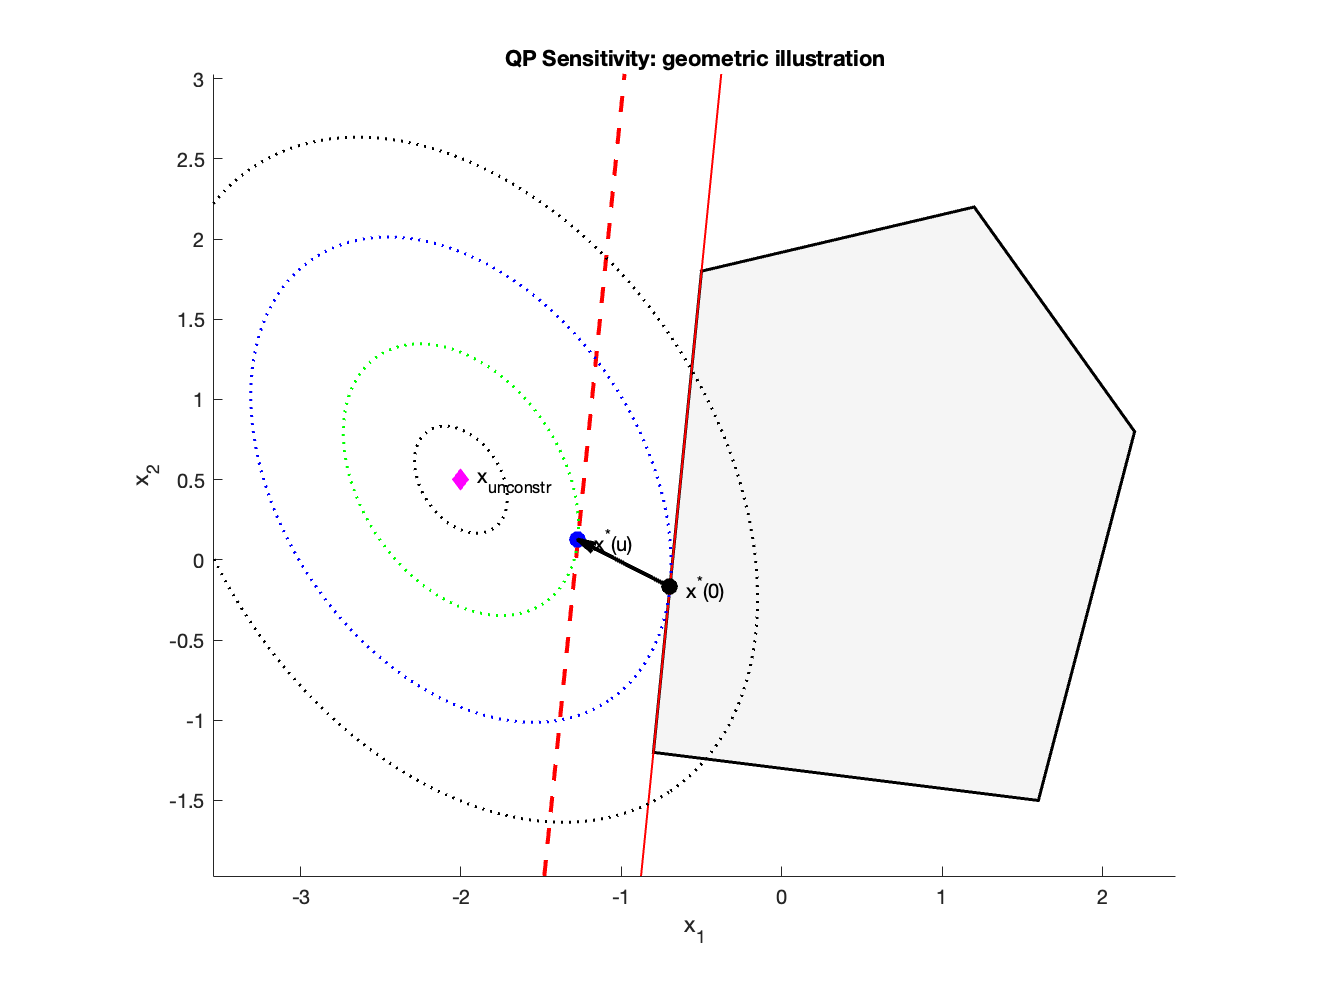
\includegraphics[width=0.9\linewidth]{illustration}
			\caption{Sensitivity w.r.t. linear constraint r.h.s. perturbation}
			\label{fig:illustration}
		\end{figure}
		
		
	\end{flushleft}
\end{frame}



\begin{frame}{Sensitivity: Perturbation in Constraint Normal}
	\begin{flushleft}
		
		Consider the problem with perturbed constraint direction:
		\begin{equation*}
			\begin{aligned}
				\min_x \quad & f(x) \\
				\text{s.t.} \quad & (a + u)^\top x \le b.
			\end{aligned}
		\end{equation*}
		
		Define the value function $v(u) = f(x^*(u))$ and Lagrangian
		\begin{equation*}
			\mathcal{L}(x,\lambda,u) = f(x) + \lambda \big((a+u)^\top x - b\big).
		\end{equation*}
		
		From the envelope theorem:
		\begin{equation*}
			\frac{dv}{du} = \frac{\partial \mathcal{L}}{\partial u}(x^*, \lambda^*, u) = \lambda^* x^*.
		\end{equation*}
		
		
	\end{flushleft}
\end{frame}


\begin{frame}{Sensitivity: Perturbation in Cost}
	\begin{flushleft}
		
		Consider the problem with perturbed cost:
		\begin{equation*}
			\begin{aligned}
				\min_x \quad & \tfrac{1}{2} x^\top Q x + (q+u)^\top x \\
				\text{s.t.} \quad & a^\top x \le b.
			\end{aligned}
		\end{equation*}
		
		Define the value function $v(u) = f(x^*(u), u)$ and Lagrangian
		\begin{equation*}
			\mathcal{L}(x,\lambda,u) = \tfrac{1}{2} x^\top Q x + (q+u)^\top x + \lambda (a^\top x - b).
		\end{equation*}
		
		From the envelope theorem:
		\begin{equation*}
			\frac{dv}{du} = \frac{\partial \mathcal{L}}{\partial u}(x^*, \lambda^*, u) = x^*.
		\end{equation*}
		
		The sensitivity equals the optimal solution: perturbing the linear cost shifts the optimal value at a rate given directly by $x^*$.
		
	\end{flushleft}
\end{frame}






\begin{frame}{Further reading}
	\begin{flushleft}
		
		\begin{itemize}
			\item \bref{https://www.stat.cmu.edu/~ryantibs/convexopt-F16/scribes/kkt-scribed.pdf}{Convex Optimization, Lecture 12: KKT conditions, Ryan Tibshirani.}
			
			\item \bref{https://people.eecs.berkeley.edu/~elghaoui/Teaching/EE227A/lecture13.pdf}{EE 227A: Convex Optimization and Applications, Lecture 13: Optimality Conditions for Convex Problems, Laurent El Ghaoui.}
			
			\item \bref{https://youtu.be/uh1Dk68cfWs?si=rHb-bFyrDeqkJo_I}{The Karush–Kuhn–Tucker (KKT) Conditions (video). Visually Explained.}
		\end{itemize}
		
		
		
		
		
		
	\end{flushleft}
\end{frame}






\myqrframe



\end{document}
